\documentclass{article}
\usepackage[english]{babel}
\usepackage{geometry,amsmath,amssymb,graphicx,wasysym,xcolor,theorem}
\geometry{top=17mm, left=15mm, left=15mm, bottom=17mm, right=15mm}

%%%%%%%%%% Start TeXmacs macros
\catcode`\<=\active \def<{
\fontencoding{T1}\selectfont\symbol{60}\fontencoding{\encodingdefault}}
\catcode`\>=\active \def>{
\fontencoding{T1}\selectfont\symbol{62}\fontencoding{\encodingdefault}}
\newcommand{\nobracket}{}
\newcommand{\tmaffiliation}[1]{\\ #1}
\newcommand{\tmcolor}[2]{{\color{#1}{#2}}}
\newcommand{\tmdummy}{$\mbox{}$}
\newcommand{\tmmathmd}[1]{\ensuremath{#1}}
\newcommand{\tmop}[1]{\ensuremath{\operatorname{#1}}}
\newcommand{\tmtextbf}[1]{\text{{\bfseries{#1}}}}
\newcommand{\tmtextit}[1]{\text{{\itshape{#1}}}}
\newenvironment{descriptioncompact}{\begin{description} }{\end{description}}
\newtheorem{definition}{Definition}
\newcounter{nndefinition}
\def\thenndefinition{\unskip}
\newtheorem{definition*}[nndefinition]{Definition}
\newcounter{nnexample}
\def\thennexample{\unskip}
{\theorembodyfont{\rmfamily}\newtheorem{example*}[nnexample]{Example}}
\newcounter{nnnote}
\def\thennnote{\unskip}
{\theorembodyfont{\rmfamily}\newtheorem{note*}[nnnote]{Note}}
%%%%%%%%%% End TeXmacs macros

\begin{document}

\title{Econometrics I}

\author{
  Christopher fu
  \tmaffiliation{\tmtextit{Verison:} September 23, 2024}
}

\maketitle

{\tableofcontents}

\

\section{Statistical Inference}

\[ x : X \sim p(x|\theta) \]
$\theta$ is the parameter setting the shape of the distribution.

\begin{definition}
  \textbf{\color{blue}Point Estimator} $\delta(X)$
  
  A mapping $\delta$ from sample space of $X$ to the parameter space $\Theta$:
  $\delta : X \rightarrow \Theta$
  
  Given $X$, what's the best $\Theta$. $\delta(x)$ is an estimate.
\end{definition}

\subsection{Methods to get $\delta(X)$}

\subsubsection{LS Estimation}

\[ X_1 \sim p(x|\theta), \quad \mathbb{E}[X_1|\theta] = \theta, \quad X_1|\theta \sim N(0, 1) \]
Point estimator $\hat{\theta}$ is the argument that minimizes the objective function
\[ \hat{\theta}_{\text{LS}} = \arg \min_{\theta} \sum_{i=1}^n (x_i - \theta)^2 \]
where we assume that $\theta = \mathbb{E}[x_i|\theta]$. Using the First Order Condition (FOC) to solve, we have
\[ \frac{\partial ()}{\partial \theta} = \sum_{i=1}^n -2(x_i - \theta) = 0 \]
We get $\hat{\theta}_{\text{LS}} = \frac{1}{n} \sum_{i=1}^n x_i$

\subsubsection{Method of Moments}

Find $\hat{\theta}$ such that
\[ \mathbb{E}[X|\hat{\theta}_{\text{MM}}] = \frac{1}{n} \sum_{i=1}^n x_i \]
Or, such that
\[ \mathbb{E}[X^2|\theta]_{\theta = \hat{\theta}_{\text{MM}}} = \frac{1}{n} \sum_{i=1}^n x_i^2 \]
$\mathbb{V}[X|\theta] = 1$, thus $\mathbb{E}[X^2|\theta] = \mathbb{V}[X|\theta] + (\mathbb{E}[X|\theta]^2) = 1 + \theta^2$. 
\[ 1 + \hat{\theta}_{\text{MM}}^2 = \frac{1}{n} \sum_{i=1}^n x_i^2 \]

We get
\[ \hat{\theta}_{\text{MM}} = \sqrt{\frac{1}{n} \sum_{i=1}^n x_i^2 - 1} \]
\begin{note*}
  Choose $\hat{\theta}_{\text{MM}}$ s.t. $\mathbb{E}[h(X)|\theta]$ under $\theta = \hat{\theta}_{\text{MM}}$ is the mean of samples $\frac{1}{n} \sum_{i=1}^n x_i^2$.
\end{note*}

\subsubsection{Maximum Likelihood}

\[ \hat{\theta}_{\text{ML}} = \arg \max_{\theta} \mathcal{L}(\theta|x) \]
where
\[ \mathcal{L}(\theta|x) = p(x|\theta) \]
is the PDF of the RV $X|\theta$.

\begin{note*}
  Specify the whole distribution.
\end{note*}

With $X$ as i.i.d. distribution, we have
\begin{align*}
  \mathcal{L}(\theta|x) & = p(x|\theta) \\
  & = \prod_{i=1}^n p(x_i|\theta) \\
  & = \prod_{i=1}^n (2\pi\sigma^2)^{-\frac{1}{2}} \exp \left\{ -\frac{1}{2} \left( \frac{x_i - \mu}{\sigma} \right)^2 \right\} \\
  & = (2\pi)^{-\frac{n}{2}} \exp \left\{ -\frac{1}{2} \sum (x_i - \mu)^2 \right\} \\
  & \sim N(0, \sigma^2)
\end{align*}
Then, let's define $\ell(\theta|x) = \log \mathcal{L}(\theta|x) = -\frac{n}{2} \log(2\pi) -\frac{1}{2} \sum (x_i - \mu)^2$
\[ \hat{\theta}_{\text{ML}} = \frac{1}{n} \sum_{i=1}^n x_i = \hat{\theta}_{\text{MM}} = \hat{\theta}_{\text{LS}} \]
\begin{align*}
  \hat{\theta}_{\text{ML}} & = \arg \max_{\theta} c - \frac{1}{2} \sum (x_i - \mu)^2\\
  & = \arg \min_{\theta} \sum (x_i - \mu)^2
\end{align*}
\begin{definition}
  $\delta(X)$ is \underline{unbiased} if $\mathbb{E}[\delta(X)|\theta] = \theta$.
\end{definition}

e.g. $\hat{\theta} = \frac{1}{n} \sum_{i=1}^n X_i$ is unbiased because
\begin{align*}
  \mathbb{E}[\hat{\theta}|\theta] & = \mathbb{E}\left[\frac{1}{n} \sum_{i=1}^n X_i|\theta \right] \\
  & = \frac{1}{n} \mathbb{E}\left[\sum X_i \right]\\
  & = \frac{1}{n} \sum \mathbb{E}[X_i]\\
  & = \theta
\end{align*}
However, $\widehat{\theta_{*}} = \frac{1}{n-1} \sum_{i=1}^n X$ is biased, because
\begin{align*}
  \mathbb{E}[\widehat{\theta_{*}}|\theta] & = \mathbb{E}\left[\frac{1}{n-1} \sum_{i=1}^n X_i|\theta \right] \\
  & = \frac{1}{n-1} \mathbb{E}\left[\sum X_i \right]\\
  & = \frac{n}{n-1} \theta\\
  & \neq \theta
\end{align*}
For the variance,
\[ \mathbb{V}[\hat{\theta}|\theta] = \mathbb{V}\left[\frac{1}{n} \sum_{i=1}^n X_i \right] = \frac{1}{n^2} \sum_{i=1}^n \mathbb{V}[X_i|\theta] = \frac{1}{n} \]
and,
\[ \mathbb{V}[\hat{\theta}_{*}|\theta] = \mathbb{V}\left[\frac{n}{n-1} \hat{\theta} \right] = \frac{n^2}{(n-1)^2} \mathbb{V}[\hat{\theta}] = \frac{n}{(n-1)^2} \]
To get the estimation of $\mathbb{E}$ and $\mathbb{V}$, we have to assume the mean and variance of the distribution.

Under $X_i|\theta \sim N(0, 1)$, we have $\hat{\theta} = \frac{1}{n} \sum X_i \sim N\left(0, \frac{1}{n} \right)$.

\subsection{Asymptotic Properties}

\begin{definition}
  Point estimator $\delta(X)$ is \underline{consistent} if $\delta(X) \overset{p}{\rightarrow} \theta$.
\end{definition}

By Weak Law of Large Numbers (WLLN),
\[ \hat{\theta} = \frac{1}{n} \sum X_i \overset{p}{\rightarrow} \mathbb{E}[X] = \theta \]
Now let's look at $\hat{\theta}_{*}$ again,
\[ \hat{\theta} = \frac{1}{n-1} \sum X_i = \frac{n}{n-1} \frac{1}{n} \sum X_i = \frac{n}{n-1} \mathbb{E}[X] = \frac{n}{n-1} \hat{\theta} \overset{p}{\rightarrow} \theta \]
as $\lim_{n \rightarrow \infty} \frac{n}{n-1} = 1$ and $\hat{\theta} \overset{p}{\rightarrow} \theta$. Slutsky's theorem tells us that we can form the limit of their product as the product of the limits.

Central Limit Theorem (CLT):
\begin{align*}
  & \sqrt{n} \frac{\frac{1}{n} \sum X_i - \mathbb{E}[X_i]}{\sqrt{\mathbb{V}[X_i]}} \overset{p}{\rightarrow} N(0, 1) \\
  \Rightarrow & \sqrt{n} \frac{\overline{X_n} - \mu}{\sigma} \overset{d}{\rightarrow} N(0, 1) \text{ Set the variance to 1} \\
  \Rightarrow & \sqrt{n} (\hat{\theta} - \theta) \overset{d}{\rightarrow} N(0, 1) \\
  \Rightarrow & \sqrt{n} (\hat{\theta} - \theta) \overset{\text{approx}}{\sim} N(0, 1) \text{ in our finite sample of } n \\
  \Rightarrow & (\hat{\theta} - \theta) \sim N\left(0, \frac{1}{n}\right) \\
  \Rightarrow & \hat{\theta} \overset{\text{approx}}{\sim} N\left(\theta, \frac{1}{n}\right) 
\end{align*}

\textbf{RECALL}: Statistical inference given $x$, what can we say?
\begin{description}
  \item[] Point inference, best guess for $\theta$
  \item[] Hypothesis testing, is $\theta$ larger than 1 or not?
  \item[] Interval inference, give an interval where you are sure that $\theta$ lies in.
\end{description}


\section{Hypothesis Testing}

\begin{definition}
  \textbf{\textcolor{blue}{Null Hypothesis}}
  
  The null hypothesis $\mathcal{H}_0$ is the set $\theta = \theta_0$ or $\beta
  \in \mathcal{B}_0$.
  
  Or, we denote it as:
  \[ \mathcal{H}_0 : \theta \in \Theta_0 \]
  For econometrics, we usually set $\mathcal{H}_0 : \beta = 0$.
\end{definition}

\begin{definition}
  \textbf{\textcolor{blue}{Alternative Hypothesis}}
  
  The alternative hypothesis $\mathcal{H}_1$ is the set $\{ \theta \in \Theta
  : \theta \neq \theta_0 \}$ or $\{ \beta \in \mathcal{B}  : \beta \notin
  \mathcal{B}_0 \}$.
  
  Or, we denote it as:
  \[ \mathcal{H}_1 : \theta \in \Theta_1 \]
  For econometrics, we usually set $\mathcal{H}_1 : \beta \neq 0$. Often
  $\Theta_1$ is the complement of $\Theta_0$.
\end{definition}

\begin{note}
  Point estimator of $\mathbb{1} \{ \theta \in \Theta_0 \}$ (if $\theta \in
  \Theta_0$, the function equals 1).
\end{note}

\begin{center}
\begin{tabular}{|c|c|c|}
  \hline
  & $\mathcal{H}_0$ is true & $\mathcal{H}_0$ is false\\
  \hline
  Accept $\mathcal{H}_0$ & $\checkmark$: $1 - \alpha$ & $\times$: $1 - \beta$\\
  \hline
  Reject $\mathcal{H}_0$ & $\times$: $\alpha$ & $\checkmark$: $\beta$\\
  \hline
\end{tabular}
\end{center}

$\alpha$ is the Type I error, $1 - \beta$ is the Type II error.

\begin{definition}
  A hypothesis test $\varphi \in \{0, 1\}$ is a rule that specifies when we
  reject and when we accept (do not reject) $\mathcal{H}_0$, with $\varphi =
  0$ indicating rejection.
\end{definition}

\begin{definition}
  \textbf{Power Function}
  \[ \beta (\theta) = \mathbb{P} [\text{rejecting} | \theta \text{ is}
     \text{ true}] = \mathbb{P} [\varphi = 0 | \theta] \]
\end{definition}

\begin{definition}
  \textbf{Size of a test}
  
  The size of a test is $\alpha$ if $\underset{\theta \in \Theta_0}{\sup}
  \beta (\theta_0) = \alpha$, $\alpha \in (0, 1)$.
\end{definition}

\textit{Generic form:}
\[ \varphi (x ; \alpha) = \mathbb{1} \{ T (x) < c_{\alpha} \} \]

\subsection{T-test}

\begin{definition}
  Suppose $\hat{\theta} | \theta \sim N (\theta, v^2)$, and we are
  testing a point hypothesis $\mathcal{H}_0 : \theta = \theta_0$. Under the
  alternative $\mathcal{H}_1 : \theta \neq \theta_0$, the two-sided t-test is
  \[ \varphi_t (x) = \mathbb{1} \left\{ \left| \frac{\hat{\theta} -
     \theta_0}{v} \right| < c \right\} \]
\end{definition}

\begin{note}
  The test-statistic $T (X) = \left| \frac{\hat{\theta} - \theta_0}{v}
  \right|$ is a function of data $X$ because our estimator $\theta$,
  $\hat{\theta}$, is a function of $X$.
\end{note}

\begin{example}
  Let $X | \theta \sim N (\theta, v^2)$, under $\mathcal{H}_0 :
  \hat{\theta} \sim N (\theta_0, v^2)$ $\rightarrow$ $\frac{\hat{\theta} -
  \theta_0}{v} \sim N (0, 1)$
\end{example}

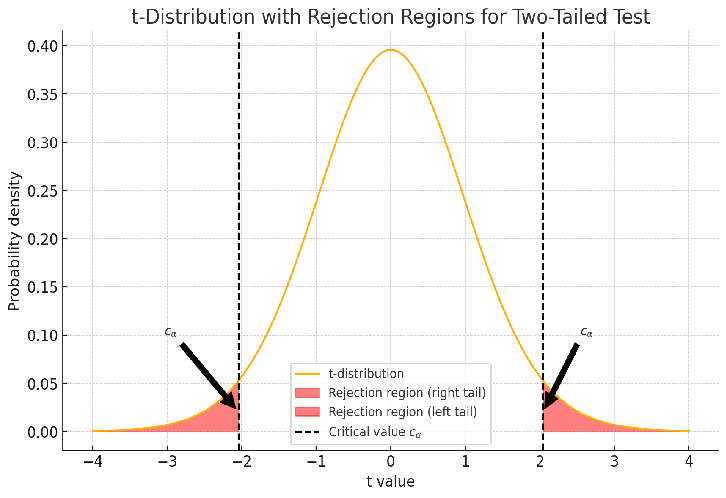
\includegraphics[width=\textwidth]{Econometrics-1.pdf}

\begin{align*}
  \beta (\theta) & = \mathbb{P} [\text{rejecting} | \theta \text{ is}
  \text{ true}]\\
  & = \mathbb{P} [\varphi = 0 | \theta]\\
  & = \mathbb{P} [T (X) > c_{\alpha} | \theta]\\
  & = \mathbb{P} \left[ \left| \frac{\hat{\theta} - \theta_0}{v} \right| >
  c_{\alpha} | \theta \right]\\
  & = 1 - \mathbb{P} \left[ \left| \frac{\hat{\theta} - \theta_0}{v}
  \right| \leq c_{\alpha} | \theta \right]\\
  & = 1 - \mathbb{P} \left[ - c_{\alpha} \leq \frac{\hat{\theta} -
  \theta_0}{v} \sim N (0, 1) \leq c_{\alpha} | \theta \right]\\
  & = 1 - \left( \mathbb{P} \left[ \frac{\hat{\theta} - \theta_0}{v} \leq
  c_{\alpha} | \theta \right] - \mathbb{P} \left[
  \frac{\hat{\theta} - \theta_0}{v} \leq - c_{\alpha} | \theta
  \right] \right)\\
  & = 1 - [\Phi (c_{\alpha}) - \Phi (- c_{\alpha})]\\
  & = 1 - [\Phi (c_{\alpha}) - (1 - \Phi (c_{\alpha}))]\\
  & = 2 - 2 \Phi (c_{\alpha})\\
  & = \alpha
\end{align*}

Under $\alpha = 0.05$, we get $c_{\alpha} = 1.64$, $\alpha = 0.1$, we get
$c_{\alpha} = 1.96$.

To compute the power of this test, we need to think about what happens if
$\mathcal{H}_0$ is false. Assuming that $\tilde{\theta}$ is the true value of
$\theta$.

\begin{align*}
  \beta (\tilde{\theta}) & = \mathbb{P} [\text{rejecting} |
  \widetilde{\theta} \text{ is true}]\\
  & = \mathbb{P} [\varphi = 0 | \widetilde{\theta}]\\
  & = \mathbb{P} [T (X) > c_{\alpha} | \widetilde{\theta}]\\
  & = \mathbb{P} \left[ \left| \frac{\hat{\theta} - \theta_0}{v} \right| >
  c_{\alpha} | \widetilde{\theta} \right]
\end{align*}

To find this, under $\tilde{\theta}$ is true, $\tilde{\theta} \sim N
(\tilde{\theta}, v^2)$, $\hat{\theta} - \tilde{\theta} \sim N (0, v^2)$,
$\hat{\theta} - \theta_0 \sim N (\tilde{\theta} - \theta_0, v^2)$,
$\frac{\hat{\theta} - \theta_0}{v} \sim N (\tilde{\theta} - \theta_0, 1)$,
$\frac{\hat{\theta} - \theta_0}{v} - (\tilde{\theta} - \theta_0) \sim N (0,
1)$

So,
\begin{align*}
  \beta (\tilde{\theta}) & = \mathbb{P} \left[ \left| \frac{\hat{\theta} -
  \theta_0}{v} \right| > c_{\alpha} | \widetilde{\theta}
  \right]\\
  & = 1 - \mathbb{P} \left[ \left| \frac{\hat{\theta} - \theta_0}{v}
  \right| \leq c_{\alpha} | \theta \right]\\
  & = 1 - \mathbb{P} \left[ - c_{\alpha} \leq \frac{\hat{\theta} -
  \theta_0}{v} \leq c_{\alpha} | \theta \right]\\
  & = 1 - \mathbb{P} [- c_{\alpha} - (\tilde{\theta} - \theta_0) \leq z
  \sim N (0, 1) \leq c_{\alpha} - (\tilde{\theta} - \theta_0)]\\
  & = 1 - (\Phi [c_{\alpha} - (\tilde{\theta} - \theta_0)] - \Phi [-
  c_{\alpha} - (\tilde{\theta} - \theta_0)])
\end{align*}

The higher the probability of wrongly accepting (or failing to reject)
$\mathcal{H}_0$. It is common to be rather conservative (i.e. erring on the
side of not rejecting $\mathcal{H}_0$) and report test results for sizes of
10\%, 5\% and 1\%.

\subsection{Likelihood Ratio Test}

\begin{definition}
  \[ \varphi_{\text{LR}} (x) = \mathbb{1} \left\{ \frac{\underset{\theta \in
     \Theta_1}{\sup} p (x | \theta)}{\underset{\theta \in
     \Theta_0}{\sup} p (x | \theta)} < c_{\alpha} \right\} \]
  $T_{\text{LR}} (X) = \frac{\underset{\theta \in \Theta_1}{\sup} p (x |
  \theta)}{\underset{\theta \in \Theta_0}{\sup} p (x | \theta)}$.
\end{definition}

So, if there are points in $\Theta_0$ for which observed $x$ is more likely
than points in $\Theta_1$, the ratio is small --- the test is likely to accept
$\mathcal{H}_0$.

Under $\mathcal{H}_0 : \theta = \theta_0$ and the alternative $\mathcal{H}_1 :
\theta \neq \theta_0$,
\[ \varphi_{\text{LR}} (x) = \mathbb{1} \left\{ \frac{p (x |
   \hat{\theta}_{\text{ML}})}{p (x | \theta_0)} < c \right\} \]

\begin{example}
  $\{ x_i \}_{i = 1}^n$, $x_i | \theta \sim N (\theta, 1)$,
  \[ p (x | \theta) = \prod_i p (x_i | \theta) = (2
     \pi)^{- \frac{1}{2}} \exp \left\{ - \frac{1}{2} (x - \theta)^2 \right\}
  \]
  if $n = 1$. As $x = \hat{\theta}$, $p (x | \hat{\theta}) = (2
  \pi)^{- \frac{1}{2}}$
  \[ T (x) = \frac{p (x | \hat{\theta}_{\text{ML}})}{p (x |
     \theta_0)} = \frac{(2 \pi)^{- \frac{1}{2}} \exp \left\{ -
     \frac{1}{2} (x - \hat{\theta})^2 \right\}}{(2 \pi)^{- \frac{1}{2}} \exp
     \left\{ - \frac{1}{2} (x - \theta_0)^2 \right\}} = \exp \left\{
     \frac{1}{2} (x - \theta_0)^2 \right\} \]
  as $x = \hat{\theta}$.
  \[ \varphi_{\text{LR}} = \mathbb{1} \left\{ \exp \left\{ \frac{1}{2} (x -
     \theta_0)^2 \right\} < c_{\alpha} \right\} \]
\end{example}

\begin{align*}
  \alpha & = \mathbb{P} \{ \text{Reject} | \theta_0 \text{ is}
  \text{ actually true} \}\\
  & = \mathbb{P} \left\{ \exp \left\{ \frac{1}{2} (x - \theta_0)^2 \right\}
  \geq c_{\alpha} | \theta_0 \right\}\\
  & = \mathbb{P} \{ (x - \theta_0)^2 \geq 2 \log c_{\alpha} |
  \theta_0 \}\\
  & = 1 - \mathbb{P} \left\{ (x - \theta_0)^2 <
  2 \log c_{\alpha} | \theta_0 \right\}
\end{align*}

If $x \sim N (\theta_0, 1)$, $(x - \theta_0)^2 \sim \chi_{1}^2$

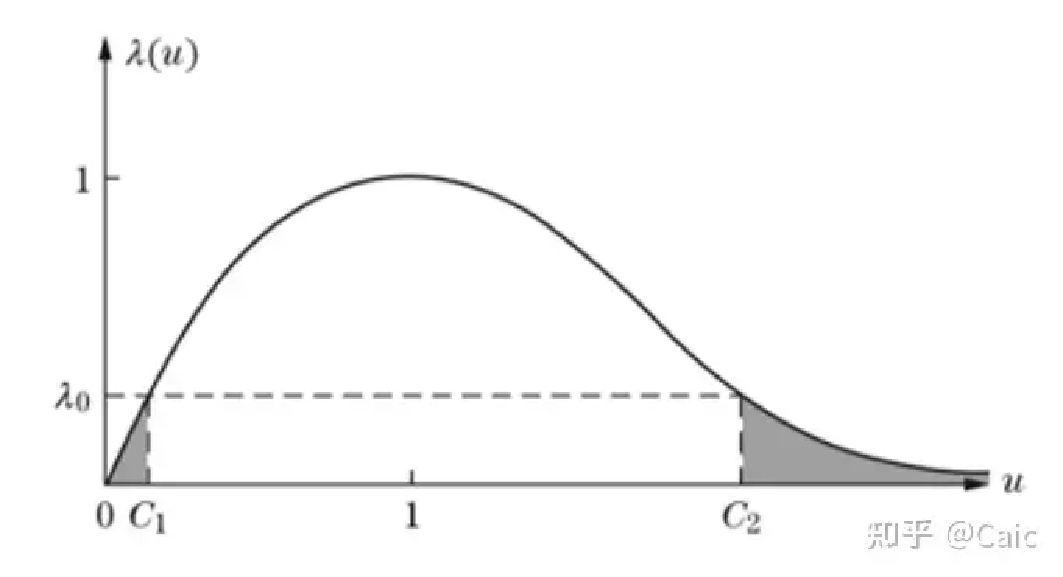
\includegraphics[width=\textwidth]{Econometrics-2.pdf}

\begin{note}
  \textbf{\textcolor{red}{Uniformly most powerful test}} Highest probability
  of rejection, of wrong acceptance.
\end{note}

\[ \varphi (x) = \mathbb{1} \{ T (x) < c_{\alpha} \} \]
\[ \alpha = \mathbb{P} \{ T (x) > c_{\alpha} | \theta_0 \} 
   (\text{reject rule}) \]

\textbf{Numerical Hypothesis Testing}

\begin{enumerate}
  \item For $m = 1 : M$, simulate data $x^m \sim N (\theta_0, 1)$, supposing
  $\theta_0$ to be true under $\mathcal{H}_0$.
  
  \item Result $\{ T (x^m) \}_{m = 1}^M$
  
  \item Conduct test, using your actual data $X$, compute $T (x)$, and see
  whether $T (x) < c$
\end{enumerate}

Small $p\text{-value}$ means $\mathcal{H}_0$ is likely to be rejected,
larger $p\text{-value}$ means it's likely to be true.

\subsection{Coverage Sets}

\textbf{Frequentist Confidence Sets}

A confidence set $C (X) \subseteq \Theta$ is a (random) set that should cover
the true $\theta$ with a prespecified probability:
\[ \underset{\theta \in \Theta}{\inf} \mathbb{P} [\theta \in C (X) |
   \theta] = 1 - \alpha \]
\[ C (x) = \{ \theta_0 \in \Theta : \varphi (x ; \theta_0) = 1 \} \]
contains all the values of $\theta_0$ that we would accept.

Consider $\mathcal{H}_0 : \theta = \theta_0$ vs. $\mathcal{H}_1 : \theta \neq
\theta_0$, $\varphi_{\alpha} (x) = \mathbb{1} \{ T (x) < c_{\alpha ; \theta_0}
\}$.

\begin{example}
  T-test: $T (x) = \left| \frac{\hat{\theta} - \theta_0}{v} \right|$
  $\Rightarrow$ $\varphi \{ x ; \theta_0, \alpha \} = \mathbb{1} \{ T (x) < c
  \}$
  \begin{align*}
    C (x) & = \{ \theta_0 \in \Theta, \varphi \{ x ; \theta_0, \alpha \} = 1
    \}\\
    & = \left\{ \theta_0 \in \Theta, \left| \frac{\hat{\theta} -
    \theta_0}{v} \right| < c \right\}\\
    & = \left\{ \theta_0 \in \Theta, - c < \frac{\hat{\theta} -
    \theta_0}{v} < c \right\}\\
    & = \{ \theta_0 \in \Theta, - c v + \hat{\theta} < \theta_0 < c v +
    \hat{\theta} \}
  \end{align*}
\end{example}

\begin{example}
  LR-test: $\varphi (x ; \theta_0, \alpha) = \mathbb{1} \{ (x - \theta_0)^2 <
  \widetilde{c_{\alpha}} \}$
  \begin{align*}
    C (x) & = \{ \theta_0 \in \Theta, \varphi \{ x ; \theta_0, \alpha \} = 1
    \}\\
    & = \{ \theta_0 \in \Theta, (x - \theta_0)^2 < \widetilde{c_{\alpha}}
    \}\\
    & = \left\{ \theta_0 \in \Theta, - \sqrt{\widetilde{c_{\alpha}}} < x -
    \theta_0 < \sqrt{\widetilde{c_{\alpha}}} \right\}\\
    & = \left\{ \theta_0 \in \Theta, x - \sqrt{\widetilde{c_{\alpha}}} <
    \theta_0 < x + \sqrt{\widetilde{c_{\alpha}}} \right\}
  \end{align*}
\end{example}

\section{Least Squares Estimation of the Linear Regression Model}

\subsection{Finite Sample Properties}

\[ y_i = x'_i \beta + u \]
\[ Y = X \beta + U \]
where
\begin{equation*}
  Y = \begin{bmatrix}
    y_1\\
    \vdots\\
    y_n
  \end{bmatrix}_{n \times 1}, \quad
  X = \begin{bmatrix}
    x'_1\\
    \vdots\\
    x'_n
  \end{bmatrix}_{n \times k}, \quad
  U = \begin{bmatrix}
    u_1\\
    \vdots\\
    u_n
  \end{bmatrix}_{n \times 1}
\end{equation*}

\textbf{Assumption 1} (Independent Sampling). Observations $z_i = \{ y_t, x_i \}_{i = 1}^n$ are independent across $i$.

\textbf{Assumption 2} (Full rank). The matrix $X'X = \sum x_i x'_i$ is of full rank.

\textbf{Assumption 3} (Conditional Independence). $\mathbb{E}[u_i | x_i] = 0$.

$\mathbb{E}[y_i] = \mathbb{E}[x'_i \beta + u_i | x_i] = \mathbb{E}[x'_i \beta | x_i] + \mathbb{E}[u_i | x_i] = x'_i \beta$

\textbf{Assumption 4} (Homoskedasticity). $\mathbb{V}[u_i | x_i] = \sigma^2$ for all $i$.

$\mathbb{V}[y_i] = \mathbb{V}[x'_i \beta + u_i | x_i] = \sigma^2$

The OLS estimator:
\[ \hat{\beta}_{\text{OLS}} = \arg\min_{\beta \in \mathbb{R}^k} 
   \sum u_i^2 = \arg\min_{\beta \in \mathbb{R}^k} \sum_{i = 1}^n
   (y_i - x'_i \beta)^2 = \arg\min_{\beta \in \mathbb{R}^k} (Y - X
   \beta)'(Y - X \beta) \]
   
\begin{align*}
  \frac{\partial (Y - X \beta)'(Y - X \beta)}{\partial \beta} &= X'(Y - X
  \beta) = 0\\
  &\Rightarrow X'Y - X'X\beta = 0\\
  &\Rightarrow (X'X)^{-1}X'Y = \hat{\beta}
\end{align*}

\[ \hat{Y} = X\hat{\beta} = X(X'X)^{-1}X'Y = P_X Y \]
where $P_X = X(X'X)^{-1}X'$ is the projection matrix.
\[ y = x\hat{\beta} + \hat{u} \rightarrow y = \hat{y} + \hat{u} \]
thus,
\[ \hat{U} = Y - \hat{Y} = Y - P_X Y = (I - P_X)Y = M_X Y \]
where $M_X$ is another projection matrix.
\[ Y = P_X Y + M_X Y = (P_X + M_X)Y \]

$P_X$ and $M_X$ are idempotent: $P_X = P'_X$ and $P_X P_X = P_X$, and are orthogonal to each other: $P_X M_X = M_X P_X = 0$.

The total sum of squares (SST) is given by:
\[ \sum_{i = 1}^n y_i^2 = Y'Y \]
It measures the variability in $y_i$ across observations $i$.

We can decompose it into the explained sum of squares (SSE) and the residual sum of squares (SSR)
\begin{align*}
  \text{SST} = Y'Y &= (P_X Y + M_X Y)'(P_X Y + M_X Y)\\
  &= Y'P_X P_X Y + Y'P_X M_X Y + Y'M_X P_X Y + Y'M_X M_X Y \\
  &= Y'P_X P_X Y + Y'M_X M_X Y\\
  &= \hat{Y}'\hat{Y} + \hat{U}'\hat{U}\\
  &= \text{SSE} + \text{SSR}
\end{align*}

Based on that, we get the $R^2$-statistic as a measure of how well $X$ accounts for the variation in $Y$ in the linear regression model:
\[ R^2 = \frac{\hat{Y}'\hat{Y}}{Y'Y} = 1 - \frac{\hat{U}'\hat{U}}{Y'Y}
   \in [0, 1] \left(\frac{\text{SSE}}{\text{SST}} = 1 - \frac{\text{SSR}}{\text{SST}}\right) \]

Look at \textbf{Assumption 3} again, it always gives product have intercept $x_{i1} = 1$.
\begin{align*}
  \mathbb{E}[\hat{\beta} | X] &= \mathbb{E}[(X'X)^{-1}X'Y | X]\\
  &= \mathbb{E}[(X'X)^{-1}X'(X\beta + U) | X]\\
  &= \mathbb{E}[\beta | X] + \mathbb{E}[(X'X)^{-1}X'U | X]\\
  &= \beta + (X'X)^{-1}X'\mathbb{E}[U | X]\\
  &= \beta\\
  \Rightarrow \mathbb{E}[\hat{\beta}] &= \mathbb{E}[\mathbb{E}[\hat{\beta} | X]] = \beta
\end{align*}

\section*{Review Session}

Sample space: $\{\Omega, \mathcal{F}, P\}$. $\Omega$ is a set of \textbf{outcomes}, $\mathcal{F}$ is a set of \textbf{events}, and $P : \mathcal{F} \rightarrow [0, 1]$ is a function that assigns probability to events. We assume that $\mathcal{F}$ is a $\sigma$-\textbf{field} (or $\sigma$-\textbf{algebra}). A \textbf{measure} is a nonnegatively countably additive set function: $f : \Omega \rightarrow \mathbb{R}$, with

\begin{description}[nosep]
  \item[] $f(A) \leq f(\emptyset) = 0$, for all $A \in \mathcal{F}$
  \item[] if $A_i \in \mathcal{F}$ is a countable sequence of disjoint sets, then
  \[ f(\cup_i A_i) = \sum_i f(A_i) \]
\end{description}

If $f(\Omega) = 1$, we call $f$ a \textbf{probability measure}. Usually, this $f$ is denoted by $p$ or $P$.

\begin{definition}
  \textbf{Kurtosis} (峰度) $\mathbb{E}[(x - \mu)^4]$
\end{definition}

\

\end{document}
